\documentclass[dvipdfmx]{jsarticle}
\usepackage{okumacro,plext}
\usepackage{natbib}
\usepackage{url}
\usepackage{txfonts}
\usepackage[utf8]{inputenc}
\usepackage[T1]{fontenc}
%\usepackage{my_resume}
\usepackage{graphicx,wrapfig}
%\usepackage[greek,english]{babel}
%\usepackage{teubner}
%\usepackage[dvipdfm,bookmarkstype=toc=true,pdfauthor={江口聡, EGUCHI Satoshi}, pdftitle={}, pdfsubject={},pdfkeywords={},bookmarks=false, bookmarksopen=false,colorlinks=true,urlcolor=blue,linkcolor=black,citecolor=black,linktocpage=true]{hyperref}
  \AtBeginDvi{\special{pdf:tounicode EUC-UCS2}}% platex-utf8 でも OK
\author{江口聡}
%\date{}
\title{ソクラテス/プラトン}
\if0 %----------------------------------------------------------------

\fi  %----------------------------------------------------------------
\begin{document}
\maketitle


\section{ソクラテス/プラトン}

\begin{itemize}

\item ソクラテス(469 B.C.--399 B.C.)とその弟子プラトン(427 B.C.--247 B.C)。学校アカデミアを開設。
\item 一般に、プラトンの初期作品(『ソクラテスの弁明』『クリトン』など比較的短かい) では歴史的にかなり忠実なソクラテスが描かれていると考えられている。 これらの作品の多くは結論が出ないまま終る。→ 実在のソクラテスが幸福や「よい生活」についてどう考えていたのかはあきらかではない。
\item プラトンの中期以降の作品(『国家』など)では、プラトン自身の哲学がソクラテスの口を借りて語られていると考えられている。

     \end{itemize}

\begin{itemize}

   \item 冨、健康、名声などがよいものであることはたいていの人が認める。
しかし本当に求めるべきものはなにか。
\item 快楽説との戦い。
\item プラトン『リュシス』。ソフィストは人間が自分の欲するものを手にいれられないことは、当人にとってよいことではないと主張。『ゴルギアス』の登場人物カリクレス、『国家』の登場人物トラシュマコスらは快楽を手に入れることこそよく生きることであると主張。
\item ソクラテス/プラトンは正義と節制の徳を身につけるべきと主張。
\end{itemize}



\subsection{ソクラテスの主張}
\begin{itemize}
\item 身体には身体の、魂には魂の、それぞれよい状態というものが何かある。(464a)

\item   見たところ善いようだが実際にはそうではないといった状態がある。(同)

\item 医術と料理術の対比。医術が健康という善い状態を目指すのに対し、料理術は快いものを目指す。体育術と化粧法の関係も同様。 (464d--465b)政治術と弁論術。

\item   専制君主は自分の望むことをなんでもすることができるが、それが善いことであるか?

\item 「ある人が、どんなことでも自分で最善と\kenten{思った}ことをしさえすれば、たとえその人が愚か者であったとしても、それが善いことだと思うのかね?」(466e)

\item 「もしだれかが何かのために何かをするとすれば、その人は直接自分がしていることを望んでいるのではなく、そのためにそれをしている、もう一つさきのことを望んでいるのではないか。」(467d) → なにかをするひとは、すべてそれを善のためにしている。(468b)

\item 人を\kenten{不正に}死刑にする者は、不当に死刑にされるものより不幸である。人に不正な仕打ちを加えることほどその人にとって大きな災厄はない。(469b)

\item 「思いどおりにふるまうということは、その人の身のためになることがそれに伴うばあいはたしかに善きことであって、そして、それがつまり、どうやら、大きな実力があるということにほかならない。しかしそうでないばあいは、それは悪しきことであり、とるにたらぬ力しかないということになるのだ」(470a)

\item   「行為が正義にかなっているばあいには身のためになり、不正であるばあいには身の害にな
  る」 (470c)

\item 「男でも女でも、立派な善き人間は幸福であり、不正で\ruby{邪}{よこしま}な人間は不幸だというのが、ぼくの主張だ」(470e)
\end{itemize}


\subsection{カリクレスの主張}

\begin{itemize}
\item 快楽の生活こそが幸福。
\end{itemize}

\subsection{ソクラテスの反駁}

\begin{itemize}
\item 快楽と善は別。善い状態と悪い状態は対立する関係にあり、両方が同時に成立することはないが、快楽と苦痛は同時に成立する。一般に苦痛と快楽は同時に終る。ex. お腹が空いている(苦)ときに食べる(快)。(497c)

\item 善い快楽と悪い快楽がある。善い快楽は有益な快楽であり、悪い快楽は有害な快楽である。(499d) 善を追求する生き方と快楽を追求する生き方は別。(500d)
\item 身体においては規律と秩序から生まれる状態が健康や強壮さ。すぐれた魂であるためにも規律と秩序が必要。正義と節制の徳が重要。 (504d)

\end{itemize}


\section{『国家』}

\begin{itemize}

\item 『国家』での国家の三分説と魂の三分説。

\item 社会の正義=社会秩序。個人の正義=精神の健康。

\item 国家→物質的必需品を生産する労働者、
  国家を防衛する軍人、国家の社会生活を組織する支配者。


\item 個人→欲求的部分、気慨的部分、理性的部分

\item 魂の内部で葛藤があることから、魂の中に部分があることがわかる。たとえば (喉が乾いているので)あるひとが水を飲みたいと思い、また、(水が不潔なのではないかと疑って)水を飲みたくないと思う、ということから、プラトンは魂には部分があると推論。
\item ←ピタゴラス派からひきついだ魂と身体の二分説。

  「身体の健康が損なわれているとしたら、たとえ世界中のあらゆる食物と飲物、あらゆる富と権力を手に入れたとしても、ひとは人生を生きるに値しないと思うだろう。生の原理である魂が台無しになり、彼から悪徳と罪とを除去してくれると思われる一事を、すなわち我々がすでに示したような意味での正義と特の獲得を、故意に避けようとするとき、われわれはそれを生きるに値する人生と言いうるだろうか。」
\item 正しい人生は不正な人生より幸福である。

\item (1)不正なひとは自分のさまざまな欲望をなにも制限しないので彼の欲望には限度がない。しかし欲望を満しつづけることはできないので、彼は常に不満であり不幸である。

\item 不正な人(僭主的な人)の魂は「たえまなく、激しい欲望の刺によって無理やりに引っぱられ、騒ぎと悔恨でいっぱいになっているだろう」(577b)


\item (2)魂は、欲望的部分、気慨的部分、欲望的部分の三つの部分からなり、この部分はそれぞれの快楽をもつ。欲望的部分:飲食、愛欲、金銭etc。気慨的部分:勝利、優越、名声。理性的部分:知恵、真理。


\item 知恵と合理性をもつ哲学者(知を愛する者)がだけが理性の快楽と無制限な欲望や官能の快楽を比較することができる。欲望の支配下にある人間は、自分自身がもっている種類の快楽しか知らず、より高度な種類の快楽の価値を評価できない。(582a以下)

\item → 現在の状態に満足しているだけでは幸福とはいえず、より高い種類の経験をもてばいっそう幸福になることもありえる。

\item (3)知性の快楽は純粋である。一方、欲求をもったひとが快楽とみなすものは、たいてい苦痛や不快の中止にすぎず、哲学者が楽しみむのにくらべて本当ではない。幻想にもとづいた快楽はほんとうの快楽ではない。

\item 真理を知らない人びとは、身体的快楽について、「下」の状態(苦)から中間の状態に移行するだけで快楽に近づいていると感じてしまう。こうした意味で身体的な快楽は実在的ではない。

\item 「思慮や徳の経験を身につけることはしないで、お祭り騒ぎやら、そういったことばかりに馴染んでいる連中は、思うに〈下〉へ運ばれたり、〈真中〉まで逆戻りしたり、そんなふうにしながら生涯をさまようのだ。そしてその〈真中〉を越えて、真の〈上〉には、かつて眼を向けたことも、運ばれていったこともなく、また真に存在しているものによって真に見たされたことも、確実かつ純粋な〈快楽〉を味わったこともないのだ。むしろ、家畜よろしく、いつも〈下〉にばかり眼を向けて、大地や食卓に頭をうなだれながら、腹いっぱい食べ、交尾をし、身を養うのだ。そして、そういう食物の類を他からより多くもつことを目指して、たがいに鉄の角やひづめで蹴ったり、付いたり、貪欲に駆られて、殺しあうのだ。」(586a)

\end{itemize}


\nocite{プラトン田中66:国家}
\nocite{プラトン藤沢66:ゴルギアス}
\nocite{norman98:_moral_philos}
\nocite{macintyre67:_short_histor_of_ethic}
\bibliographystyle{eguchi}  
\bibliography{bib}

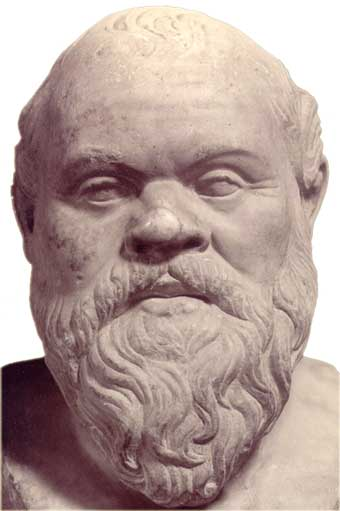
\includegraphics[width=60mm]{image/socrates.jpg}
\includegraphics[width=60mm]{images/plato.jpg}




\end{document} %----------------------------------------------------------------










%%% Local Variables:
%%% mode: japanese-latex
%%% TeX-master: t
%%% coding: utf-8
%%% End:
